\documentclass[../main.tex]{subfiles}
\begin{document}
\chapter{Integral Theorems}
\section{Green's Theorem in the Plane}
\subsection{Statement and Proof}
\begin{theorem}[Green's Theorem]
  Given an area $A \subset \R^2$ with piecewise smooth boundary $C = \partial A$ and continuously differentiable functions $P(x, y)$ and $Q(x, y)$, then:
  \label{greensTheorem}
  \[
    \int_{A} \left(\pderiv{Q}{x} - \pderiv{P}{y}\right) \d{x} \d{y} = \oint_{C} (P \d{x} + Q \d{y})
  \]
  where $C$ is traversed in the ``positive sense''.

  The ``positive sense'' usually means anti-clockwise, however there are some edge cases involving multiple boundary curves that will be discussed later.
\end{theorem}
\begin{proof}
  Initially, we assume that $A$ is a simple shape.
  This means that for each $y$ there is a single range of values of $x$, namely $x^{-}(y) \leq x \leq x^{+}(y)$.
  Likewise, for each $x$ there is a range $y^{-1}(x) \leq y \leq y^{+}(x)$.
  The diagram below shows an example $y$ and its associated range of values of $x$.
  \begin{center}
  \begin{tikzpicture}[>=stealth]
    \draw[thick, fill=gray!50, postaction={decorate}, decoration={
          markings,
          mark = between positions 0 and 1 step 0.2 with {\arrow{<}}
        }] (-1,1) to[closed, curve through = { (-0.5, 1.3) (0, 1.8) (1, 1.9) (2.5, 0) (1.2, -1.9) (0, -1.6) }] (-1, -1);
    \draw (0, -2) -- (0, 2);
    \draw (-2, 0) -- (3, 0);
    \draw[dotted, thick] (-2, -1.9) -- (3, -1.9) node[right, scale=0.8] {$y_{\text{min}}$};
    \draw[dotted, thick] (-2, 1.97) -- (3, 1.97) node[right, scale=0.8] {$y_{\text{max}}$};
    \filldraw[fill=white, draw=black] (0.55, 1.97) circle (1.5pt) node[above] {$P_1$};
    \filldraw[fill=white, draw=black] (1.1, -1.9) circle (1.5pt) node[below] {$P_2$};
    \node at (2.5, 1.3) {$C^{+}$};
    \node at (-1.3, 1.2) {$C^{-}$};
    \node at (0.6, 0.5) {$A$};

    \draw[dashed] (-0.65, 1.2) -- (2.02, 1.2);
    \fill (0, 1.2) circle (1.5pt) node[below right, scale=0.8] {$y$};
    \draw[dashed] (-0.65, 1.2) -- (-0.65, 0) node[below, scale=0.8] {$x^{-}(y)$};
    \draw[dashed] (2.02, 1.2) -- (2.02, 0) node[below, scale=0.8] {$x^{+}(y)$};
  \end{tikzpicture}
  \end{center}
  We can then divide $C$ into a right hand part $C^{+}$, on which $x = x^{+}(y)$ for each $y$ in the range $y_{\text{min}} \leq y \leq y_{\text{max}}$ and left hand part $C^{-}$ on which $x = x^{-}(y)$.
  In the above diagram, $C^{+}$ goes from $P_2 \to P_1$ and $C^{-}$ goes from $P_1 \to P_2$.

  We can now evaluate the area integral of $\pderiv{Q}{x}$:
  \begin{align*}
    \int_{A} \pderiv{Q}{x} \d{x} \d{y} &= \int_{y_{\text{min}}}^{y_{\text{max}}} \left(\int_{x^{-}(y)}^{x^{+}(y)} \pderiv{Q}{x} \d{x}\right) \d{y} \text{ by definition of area integrals} \\
                                       &= \int_{y_{\text{min}}}^{y_{\text{max}}} [Q(x^{+}(y), y) - Q(x^{-}(y), y)] \d{y} \text{ using FTC} \\
                                       &= \int_{y_{\text{min}}}^{y_{\text{max}}} Q(x^{+}(y), y) \d{y} + \int_{y_{\text{max}}}^{y_{\text{min}}} Q(x^{-}(y), y) \d{y} \\
                                       &= \int_{C^{+}} Q(x, y) \d{y} + \int_{C^{-}} Q(x, y) \d{y} \\
                                       &= \oint Q \d{y}
  \end{align*}
  Similarly, for $\pderiv{P}{y}$:
  \begin{align*}
    \int_{A} \pderiv{P}{y} \d{y} \d{x} &= \int_{x_{\text{min}}}^{x_{\text{max}}} \left(\int_{y^{-}(x)}^{y^{+}(x)} \pderiv{P}{y} \d{y}\right) \d{x} \\
                                       &= \int_{x_{\text{min}}}^{x_{\text{max}}} [P(x, y^{+}(x)) - P(x, y^{-}(x))] \d{x} \text{ using FTC} \\
                                       &= -\int_{x_{\text{max}}}^{x_{\text{min}}} P(x, y^{-}(x)) \d{x} - \int_{x_{\text{min}}}^{x_{\text{max}}} P(x, y^{+}(x)) \d{x} \\
                                       &= -\int_{C^{+}} P(x, y) \d{x} - \int_{C^{-}} P(x, y) \d{x} \\
                                       &= -\oint P \d{x}
  \end{align*}
  So for simple shapes, we are done.

  If $A$ is a more complicated shape (i.e. multiple ranges of $x$ for each $y$ and/or vice versa), then we can split it up into multiple areas $A_i$, each of which is a simple shape, and apply the calculation above to each part to obtain the same result.
  The details of this will be explained below.
\end{proof}
\begin{remark}[Result for non-simple shapes]
  \nonexaminable
  If we have split $A_i$ into disjoint areas then:
  \[
    \int_{A} \pderiv{Q}{x} \d{x} \d{y} = \sum_{i} \int_{A_i} \pderiv{Q}{x} \d{x} \d{y}
  \]
  Furthermore:
  \[
    \oint_{\partial A} Q \d{y} = \sum_{i} \oint_{\partial A_i} Q \d{y}
  \]
  Although each $\partial A_i$ contains a segment not part of the full $\partial A$, these parts cancel out as we have the same segment traversed in different directions in different parts of the shape.

  For example, the following shape has been split into two simple shapes that are infinitesimally close:
  \begin{center}
  \begin{tikzpicture}[>=stealth]
    \draw[thick, fill=gray!50, postaction={decorate}, decoration={
          markings,
          mark = between positions 0.2 and 0.8 step 0.2 with {\arrow{<}}
        }] (0.1, -0.1) to[curve through = { (-0.2, -0.5) (-1, -1) (-1.5, 0) (-0.5, 1.3) (0, 1.8) }] (0.5, 1.9);
    \draw[thick, postaction={decorate}, decoration={
          markings,
          mark = between positions 0.2 and 0.8 step 0.3 with {\arrow{>}}
        }] (0.1, -0.1) -- (0.5, 1.9);

    \begin{scope}[xscale=-1, rotate=23, xshift=-0.4cm, yshift=0.08cm]
      \draw[thick, fill=gray!50, postaction={decorate}, decoration={
            markings,
            mark = between positions 0.2 and 0.8 step 0.2 with {\arrow{>}}
          }] (0.1, -0.1) to[curve through = { (-0.2, -0.5) (-1, -1) (-1.5, 0) (-0.5, 1.3) (0, 1.8) }] (0.5, 1.9);
      \draw[thick, postaction={decorate}, decoration={
            markings,
            mark = between positions 0.2 and 0.8 step 0.3 with {\arrow{<}}
          }] (0.1, -0.1) -- (0.5, 1.9);
    \end{scope}
    \draw (0, -2) -- (0, 2);
    \draw (-2, 0) -- (3, 0);
    \node at (0, 0.9) {$L_1$};
    \node at (-0.9, -0.3) {$A_1$};
    \node at (0.75, 0.8) {$L_2$};
    \node at (0.9, -0.6) {$A_2$};
    \node[scale=0.5] at (0.8, 2.1) {Infinitesimally close};
  \end{tikzpicture}
  \end{center}
  So the sum of the integrals around the boundary of each half is:
  \begin{align*}
    \oint_{\partial A_1} Q \d{y} + \oint_{\partial A_2} Q \d{y} &= \oint_{\partial A} Q \d{y} + \int_{L_1} Q \d{y} + \int_{L_2} Q \d{y} \\
                                                                &= \oint_{\partial A} Q \d{y} + \int_{L_1} Q \d{y} - \int_{L_1} Q \d{y} \\
                                                                &= \oint_{\partial A} Q \d{y}
  \end{align*}
  We can split up $\int_{A} \pderiv{P}{y} \d{x} \d{y}$ using a similar technique and so the result follows for non-simple shapes too.
\end{remark}
\begin{example}[Area of an ellipse]
  Let $A$ be the elliptical region $\frac{x^2}{a^2} + \frac{y^2}{b^2} \leq 1$ and let $P = -\frac{1}{2}y, Q = \frac{1}{2}x$.
  $\pderiv{Q}{x} - \pderiv{P}{y} = 1$ and so:
  \[
    \int_{A} \left(\pderiv{Q}{x} - \pderiv{P}{y}\right) \d{x} \d{y} = \int_{A} 1 \d{x}\d{y} = \text{Area of A}
  \]
  By Greens theorem, this area integral will be the same as the line integral around the boundary ellipse $\partial A$.
  We can parameterise $\partial A$ using $(a \cos t, b \sin t)$, $t \in [0, 2\pi)$ and so:
  \[
    \oint_{\partial A} (P \d{x} + Q \d{y}) = \int_{0}^{2\pi} \left(-\frac{1}{2}b \sin t (-a \sin t) + \frac{1}{2}a \cos t (b \cos t)\right) \d{t} = \pi ab
  \]
  Thus the area of $A$ is $\pi ab$.
\end{example}
\subsection{Multiple Boundary Curves}
\label{greensMultipleBoundaries}
Sometimes an area might have two more more boundary curves.
In this case, we can express $A$ as:
\[
  \partial A = \bigcup_{i} C_i
\]
To use Green's theorem here, we have to traverse the outer boundary, say $C_1$, anti-clockwise, but the inner boundaries, say $C_2$ etc, clockwise.
\begin{center}
\begin{tikzpicture}[>=stealth]
  \draw[thick, fill=gray!50, postaction={decorate}, decoration={
        markings,
        mark = between positions 0 and 1 step 0.2 with {\arrow{<}}
      }] (-1,1) to[closed, curve through = { (-0.5, 1.3) (0, 1.8) (1, 1.9) (2.5, 0) (1.2, -1.9) (0, -1.6) }] (-1, -1);

  \draw[thick, fill=white, scale=0.5, postaction={decorate}, decoration={
        markings,
        mark = between positions 0 and 1 step 0.2 with {\arrow{>}}
      }] (-1,1) to[closed, curve through = { (-0.5, 1.3) (0, 1.8) (1, 1.9) (2.5, 0) (1.2, -1.9) (0, -1.6) }] (-1, -1);
  \draw (0, -2) -- (0, 2);
  \draw (-2, 0) -- (3, 0);

  \node at (2, 1.8) {$C_1$};
  \node at (0.5, 0.5) {$C_2$};
  \node at (1.5, 1) {$A$};

  \begin{scope}[xshift=6cm]
    \draw[thick, fill=gray!50, postaction={decorate}, decoration={
          markings,
          mark = between positions 0 and 1 step 0.2 with {\arrow{<}}
        }] (-1,1) to[closed, curve through = { (-0.5, 1.3) (0, 1.8) (1, 1.9) (2.5, 0) (1.2, -1.9) (0, -1.6) }] (-1, -1);

    \draw[thick, fill=gray!20, scale=0.5, postaction={decorate}, decoration={
          markings,
          mark = between positions 0 and 1 step 0.2 with {\arrow{<}}
        }] (-1,1) to[closed, curve through = { (-0.5, 1.3) (0, 1.8) (1, 1.9) (2.5, 0) (1.2, -1.9) (0, -1.6) }] (-1, -1);
    \draw (0, -2) -- (0, 2);
    \draw (-2, 0) -- (3, 0);

    \node at (2, 1.8) {$C_1$};
    \node at (0.5, 0.5) {$-C_2$};
    \node at (1.5, 1) {$A$};
    \node at (0.5, -0.3) {$A_2$};
  \end{scope}
\end{tikzpicture}
\end{center}
In the case where $P$ and $Q$ are defined in all of $A_1$, we can split the area integral over $A_1$ up into two areas.
Let $A_2$ be the interior of $C_2$ and let $A_1 = A \cup A_2$.
We can split the integral over $A_1$ up as $\int_{A_1} =  \int_{A} + \int_{A_2}$.
Then, using the standard version of Greens theorem, $\int_{A_1} = \oint_{C_1}$, and, since we must traverse the curve anticlockwise, $\int_{A_2} = \oint_{-C_2}$.
Thus $\int_{A} = \oint_{C_1} - \oint_{-C_2} = \oint_{C_1} + \oint_{C_2}$.

However, this method only works if $P$ and $Q$ are defined in all of $A_1$, whereas we are given only that they are defined in $A$.
It is quite common for integrands to be undefined at certain points so we would still like to be able to apply Green's Theorem in these cases.
In such cases, consider instead the curve $\widetilde{C}$ with cross cuts $L_1$ and $L_2$ that are arbitrarily close to each other:
\begin{center}
\begin{tikzpicture}[>=stealth]
  \draw[thick, fill=gray!50, postaction={decorate}, decoration={
        markings,
        mark = between positions 0 and 1 step 0.2 with {\arrow{<}}
      }] (-1,1) to[closed, curve through = { (-0.5, 1.3) (0, 1.8) (1, 1.9) (2.5, 0) (1.2, -1.9) (0, -1.6) }] (-1, -1);

  \draw[thick, fill=white, scale=0.5, postaction={decorate}, decoration={
        markings,
        mark = between positions 0 and 1 step 0.2 with {\arrow{>}}
      }] (-1,1) to[closed, curve through = { (-0.5, 1.3) (0, 1.8) (1, 1.9) (2.5, 0) (1.2, -1.9) (0, -1.6) }] (-1, -1);

  \node at (2, 1.8) {$\widetilde{C}$};
  \node at (1.5, 1) {$\widetilde{A}$};

  \fill (0, 0) circle (1.5pt) node[above right, scale=0.5] {Singularity};

  \fill[white] (1.1, -0.2) rectangle (2.6, 0.2);
  \draw[thick, postaction={decorate}, decoration={
        markings,
        mark = at position 0.5 with {\arrow{<}}
      }] (1.235, -0.2) -- (2.522, -0.2) node[midway, below] {$L_1$};
  \draw[thick, postaction={decorate}, decoration={
        markings,
        mark = at position 0.5 with {\arrow{>}}
      }] (1.202, 0.2) -- (2.485, 0.2) node[midway, above] {$L_2$};

  \draw (0, -2) -- (0, 2);
  \draw (-2, 0) -- (3, 0);

  \draw[thick, ->] (3.2, 0) -- (4.8, 0) node[midway, above] {Limiting};
  \begin{scope}[xshift=7cm]
    \draw[thick, fill=gray!50, postaction={decorate}, decoration={
          markings,
          mark = between positions 0 and 1 step 0.2 with {\arrow{<}}
        }] (-1,1) to[closed, curve through = { (-0.5, 1.3) (0, 1.8) (1, 1.9) (2.5, 0) (1.2, -1.9) (0, -1.6) }] (-1, -1);

    \draw[thick, fill=white, scale=0.5, postaction={decorate}, decoration={
          markings,
          mark = between positions 0 and 1 step 0.2 with {\arrow{>}}
        }] (-1,1) to[closed, curve through = { (-0.5, 1.3) (0, 1.8) (1, 1.9) (2.5, 0) (1.2, -1.9) (0, -1.6) }] (-1, -1);

    \node at (2, 1.8) {$C_1$};
    \node at (0.5, 0.5) {$C_2$};
    \node at (1.5, 1) {$\approx A$};

    \fill (0, 0) circle (1.5pt) node[above right, scale=0.5] {Singularity};

    \fill[white] (1.1, -0.05) rectangle (2.6, 0.05);
    \draw[thick, postaction={decorate}, decoration={
          markings,
          mark = at position 0.5 with {\arrow{<}}
        }] (1.239, -0.05) -- (2.517, -0.05) node[midway, below] {$L_1$};
    \draw[thick, postaction={decorate}, decoration={
          markings,
          mark = at position 0.5 with {\arrow{>}}
        }] (1.233, 0.05) -- (2.507, 0.05) node[midway, above] {$L_2$};

    \draw (0, -2) -- (0, 2);
    \draw (-2, 0) -- (3, 0);
  \end{scope}
\end{tikzpicture}
\end{center}
This encloses an area $\widetilde{A}$ and since $P$ and $Q$ are defined in all of $\widetilde{A}$, using the standard Green's Theorem $\int_{\widetilde{A}} = \oint_{\widetilde{C}}$.
In the limit as these cross cuts approach each other, $\widetilde{A}$ becomes the whole of $A$ and $\widetilde{C}$ becomes the whole of $C_1$ and $C_2$ since the cross cuts cancel out in the limit as they are integrals over the same path traversed in opposite directions.
\section{Stokes' Theorem}
\subsection{Statement and Proof}
\begin{theorem}[Stokes' Theorem]
  If $\vec{F}(\vec{x})$ is continuously differentiable vector field and $S$ is a piecewise smooth orientable \textbf{open} surface with piecewise smooth boundary curve $C= \partial S$, then:
  \label{stokesTheorem}
  \[
    \int_{S} \nabla \times \vec{F} \cdot \d{\vec{S}} = \oint_{C} \vec{F} \cdot \d{\vec{x}}
  \]
  where $C$ is traversed in the ``positive sense'' with regard to the normal on $S$.

  That is, the flux of $\nabla \times \vec{F}$ through $\vec{S}$ is equal to the line integral of $\vec{F}$ over the boundary of $S$, $C = \partial S$.
\end{theorem}
\begin{remark}
  Green's Theorem in the plane (\cref{greensTheorem}) is a special 2D case of Stoke's Theorem.

  Suppose that $S$ is a flat surface in the plane $z = 0$ and that $\vec{F} = (P, Q, 0)$.
  We then see that $\nabla \times \vec{F} = (0, 0, \pderiv{Q}{x} - \pderiv{P}{y})$ and $\d{S} = (0, 0, 1)\d{x}\d{y}$ and so by Stokes' Theorem:
  \[
    \int_{S} \left(\pderiv{Q}{x} - \pderiv{P}{y}\right) \d{x}\d{y} = \int_{S} \begin{pmatrix}
    0 \\
    0 \\
    \pderiv{Q}{x} - \pderiv{P}{y} \\
    \end{pmatrix} \cdot \begin{pmatrix}
    0 \\
    0 \\
    1 \\
    \end{pmatrix} \d{x} \d{y} =
    \oint_{C} \begin{pmatrix}
    P \\
    Q \\
    0 \\
    \end{pmatrix} \cdot \d{\vec{x}} =
    \oint_{C} (P \d{x} + Q \d{y})
  \]
  which is exactly Green's Theorem.
\end{remark}
For Stokes' Theorem, the \textit{positive sense} is defined \textbf{with regard to the normal} because the notion of ``anti-clockwise'' does not make sense for open surfaces which could be viewed from any side.

The precise rule is that if $\vec{t}$ is the tangent vector for the curve $C$ (see \cref{movingTrihedral}) and $\vec{n}$ is the normal to $S$ at the same point, then $\vec{t} \times \vec{n}$ should point away from the surface.
Note $\vec{n}$ is the \textbf{normal to the surface} and not the principal normal of $C$.
Equivalently, if I walk along $C$ with my feet on $C$ and my head in the direction of $\vec{n}$, the surface should stay on my \textbf{left}.
\begin{remark}[Right Hand Rule]
  In practice, we can instead use a simpler \textit{right hand rule}:

  If your thumb points along $\vec{n}$, your curled fingers indicate the direction $C$ should be traversed.
  This is equivalent to anticlockwise if you are looking down $\vec{n}$ towards the surface.
\end{remark}
\begin{proof}[Stokes' Theorem]
\nonexaminable
  We can prove Stokes' Theorem from Green's Theorem (\cref{greensTheorem}).
  We can parameterise $S$ using $(u, v) \in D \subset R^2$, then by the chain rule:
  \[
    \d{\vec{x}} = \pderiv{\vec{x}}{u} \d{u} + \pderiv{\vec{x}}{v} \d{v}
  \]
  and so:
  \[
    \oint_{C} \vec{F} \cdot \d{\vec{x}} = \oint_{\partial D} \vec{F} \cdot \left(\pderiv{\vec{x}}{u} \d{u} + \pderiv{\vec{x}}{v} \d{v}\right)
  \]
  Now let $P(u, v) = \vec{F}(\vec{x}(u, v)) \cdot \pderiv{\vec{x}}{u}$ and $Q(u, v) = \vec{F}(\vec{x}(u, v)) \cdot \pderiv{\vec{x}}{v}$.
  We can now apply Green's theorem in the $(u, v)$-plane to yield:
  \[
    \oint_{\partial D} \vec{F} \cdot \left(\pderiv{\vec{x}}{u} \d{u} + \pderiv{\vec{x}}{v} \d{v}\right) = \int_{D} \left(\pderiv{Q}{u} - \pderiv{P}{v}\right) \d{u} \d{v}
  \]
  We can use suffix notation to show that:
  \begin{align*}
    \nabla \times \vec{F} \cdot \d{S} &= (\nabla \times \vec{F}) \cdot \left(\pderiv{\vec{x}}{u} \times \pderiv{\vec{x}}{v}\right) \\
                                      &= \levi_{i j k} \levi_{i p q} \pderiv{F_k}{x_j} \pderiv{x_p}{u} \pderiv{x_q}{v} \\
                                      &= \pderiv{F_k}{x_j} \pderiv{x_j}{u} \pderiv{x_k}{v} - \pderiv{F_k}{x_j} \pderiv{x_k}{u} \pderiv{x_j}{v}
  \end{align*}
  We can also show using suffix notation and the chain rule that:
  \begin{align*}
    \pderiv{Q}{u} - \pderiv{P}{v} &= \pderiv{}{u}\left(\vec{F} \cdot \pderiv{\vec{x}}{v}\right) - \pderiv{}{v}\left(\vec{F} \cdot \pderiv{\vec{x}}{u}\right) \\
                                  &= \pderiv{}{x_j}\left(F_k \pderiv{x_k}{v}\right) \pderiv{x_j}{u} - \pderiv{}{x_j}\left(F_k \pderiv{x_k}{u}\right)\pderiv{x_j}{v} \\
                                  &= \pderiv{x_k}{v}\pderiv{}{x_j}(F_k) \pderiv{x_j}{u} - \pderiv{x_j}{v}\pderiv{}{x_j}(F_k) \pderiv{x_k}{u} \\
                                  &= \pderiv{F_k}{x_j} \pderiv{x_j}{u} \pderiv{x_k}{v} - \pderiv{F_k}{x_j} \pderiv{x_k}{u} \pderiv{x_j}{v}
  \end{align*}
  Thus:
  \[
    \pderiv{Q}{u} - \pderiv{P}{v} = \nabla \times \vec{F} \cdot \d{\vec{S}}
  \]
  and so the result follows.
\end{proof}
\begin{example}
  Verify Stokes' Theorem for the open surface $S$ given by $z = (x^2 + y^2)^2$, $0 \leq z \leq 1$ and the vector field $\vec{F} = (x^2 y, 0, 0)$.

  \textbf{Flux Integral}\par
  We can use cylindrical polar coordinates, and so $S$ becomes $z = \rho^4$ and:
  \[
    \vec{x} = \begin{pmatrix}
    \rho \cos \phi \\
    \rho \sin \phi \\
    \rho^4 \\
    \end{pmatrix}
  \]
  To figure out what this looks like, since the surface is radially symmetric, consider the curve $z = x^4,\ x \geq 0$ in the $(x, z)$-plane.
  The surface is then just the surface of revolution of this.

  To find the vector surface element, we can use \cref{dSFormula}:
  \[
    \d{\vec{S}} = -\begin{pmatrix}
    \cos \phi \\
    \sin \phi \\
    4 \rho^3 \\
    \end{pmatrix} \times \begin{pmatrix}
    -\rho \sin \phi \\
    \rho \cos \phi \\
    0 \\
    \end{pmatrix} \d{\rho}\d{\phi} = \begin{pmatrix}
    4\rho^4 \cos \phi \\
    4\rho^4 \sin \phi \\
    -\rho \\
    \end{pmatrix} \d{\rho}\d{\phi}
  \]
  where we chose the $-$ sign so we get the downwards-facing normal.
  Note this is not an ``outwards'' facing normal as the surface is open so does not have a notion of being inside or outside.

  Now:
  \[
    \nabla \times \vec{F} = \begin{pmatrix}
    0 \\
    0 \\
    -x^2 \\
    \end{pmatrix} = \begin{pmatrix}
    0 \\
    0 \\
    -\rho^2 \cos^2 \phi \\
    \end{pmatrix}
  \]
  and so:
  \[
    \int_{S} \nabla \times \vec{F} \cdot \d{\vec{S}} = \int_{\rho = 0}^{1} \int_{\phi = 0}^{2\pi} \rho^3 \cos^2 \phi \d{\phi} \d{\rho} = \frac{\pi}{4}
  \]

  \textbf{Boundary Integral}\par
  The boundary $C = \partial S$ is just the curve $x^2 + y^2 = 1,\ z = 1$, or in cylindrical polars $\rho = 1,\ z = 1,\ \phi \in [0, 2\pi)$.
  To figure out which direction we use, the right hand rule tells us that we must traverse $C$ in the direction of decreasing $\phi$.

  We can parameterise $C$ as $x = \cos \phi$, $y = \sin \phi$, $z = 1$ where $\phi$ decreases from $2\pi$ to $0$.
  Therefore, the line integral over $C$ is:
  \[
    \oint_{C} \vec{F} \cdot \d{\vec{x}} = \int_{2\pi}^{0} x^2 y \deriv{x}{\phi} \d{\phi} = - \int_{2\pi}^{0} \cos^2 \phi \sin^2 \phi \d{\phi} = \frac{\pi}{4}
  \]
  So they agree, as expected.
\end{example}
\subsection{Closed Surfaces}
Although we stated that Stoke's Theorem is for open surfaces, it also applies to closed surfaces $S$.
However, for a closed surface $S$, $\partial S = \emptyset$ and so the line integral over $\partial S$ is 0.
This means that:
\[
  \oiint_S \nabla \times \vec{F} \cdot \d{\vec{S}} = 0
\]
\subsection{Multiple Boundary Curves}
Similarly to how in Green's Theorem we have to consider what happens when an area has multiple boundary curves, an open surface may have multiple boundary curves.
We have to apply the right hand rule for the directions of $\vec{n}$ and the direction the curve is traversed separately for each boundary which \textit{usually} results in opposite orientations for each boundary.
\subsection{Extended Example}
\begin{remark}[Question]
  Verify Stokes' Theorem for $\vec{F}(\vec{x}) = (y, z, x^2 + y^2)$ on the hyperboloid of one sheet given by $z^2 + 1 = x^2 + 4y^2$ for $0 \leq z \leq \sqrt{3}$.
\end{remark}
To visualise this surface, consider a fixing $z$.
For a fixed $z = c$:
\[
  x^2 + 4y^2 = 1 + c^2
\]
which is an ellipse with major axis along the $x$ axis.
If we pick a larger $z = c$, then $1 + c^2$ increases and so the size of the ellipse increases with $z$.
\begin{center}
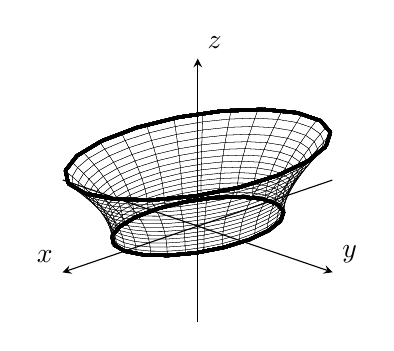
\begin{tikzpicture}
\begin{axis}[
  view={135}{20},
  axis lines=center,axis on top,
  ticks=none,set layers=default,axis equal,
  xlabel={$x$}, ylabel={$y$}, zlabel={$z$},
  xlabel style={anchor=south east},
  ylabel style={anchor=south west},
  zlabel style={anchor=south west},
  enlargelimits,
  tick align=inside,
  domain=0:2.00,
  samples=20,
  z buffer=sort,
]
  \def\a{0.8}
  \def\b{0.5}
  \def\c{0.5}
  \def\umax{1}

  \addplot3[
      mesh,
      samples=15,
      samples y=30,
      domain=0:\umax,
      domain y=0:360,
      draw=black,
      line width=0.1pt,
  ]
  (
      {\a*cosh(x)*cos(y)},
      {\b*cosh(x)*sin(y)},
      {\c*sinh(x)}
  );
  \addplot3[
      mesh,
      domain=0:360,
      samples=20,
      very thick,
      black
  ]
  (
    { \a*cos(x) },
    { \b*sin(x) },
    { 0 }
  );
  \addplot3[
      mesh,
      domain=0:360,
      samples=20,
      very thick,
      black
  ]
  (
    { \a*cosh(\umax)*cos(x) },
    { \b*cosh(\umax)*sin(x) },
    { \c*sinh(\umax) }
  );
\end{axis}
\end{tikzpicture}
\end{center}
\subsubsection{Flux Integral}
Since the normal direction was not specified, we will choose the normal to the surface that points away from the axis.

We would try cylindrical polar coordinates, but then the ranges of $\phi$ would depend on $\rho$ in a complicated way.
Instead, to parameterise the surface, we consider parametrising an ellipse for each $z$.
For $z = c$, the ellipse was:
\[
  \frac{x^2}{1 + c^2} + \frac{y^2}{\frac{1 + c^2}{4}} = 1 \to \left(\sqrt{1 + c^2}\cos \alpha, \frac{1}{2}\sqrt{1 + c^2} \sin \alpha\right),\ \alpha \in [0, 2\pi)
\]
and so we can parameterise the surface as:
\[
  \vec{x}(z, \alpha) = \left(\sqrt{z^2 + 1}\cos \alpha, \frac{1}{2}\sqrt{z^2 + 1} \sin \alpha, z\right)
\]
for $z \in [0, \sqrt{3}]$ and $\alpha \in [0, 2\pi)$.

Next, we need to find the vector surface element using \cref{dSFormula}:
\[
  \d{\vec{S}} = \pm \begin{pmatrix}
  \frac{z}{\sqrt{z^2 + 1}} \cos \alpha \\
  \frac{z}{2\sqrt{z^2 + 1}} \sin \alpha \\
  1 \\
  \end{pmatrix} \times \begin{pmatrix}
  - \sqrt{z^2 + 1} \sin \alpha \\
  \frac{1}{2} \sqrt{z^2 + 1} \cos \alpha \\
  0 \\
  \end{pmatrix} \d{z}\d{\alpha} = \pm \begin{pmatrix}
  -\frac{1}{2}\sqrt{z^2 + 1} \cos \alpha \\
  - \sqrt{z^2 + 1} \sin \alpha \\
  \frac{1}{2} z \\
  \end{pmatrix} \d{z} \d{\alpha}
\]
\begin{remark}[Advice]
  It is really worth double checking that you have taken this cross product correctly as any errors will cascade very far into your answer.
\end{remark}
We decided to use the normals pointing away from the axis, visually, we see these should all have negative $z$ component and we take the normal corresponding to the $-$ sign.

$\nabla \times \vec{F} = (2y - 1, -2x, -1)$, so on the surface:
\[
  \nabla \times \vec{F} = \left(\sqrt{z^2 + 1} \sin \alpha - 1, -2 \sqrt{z^2 + 1} \cos \alpha, -1\right)
\]
So the flux of $\nabla \times \vec{F}$ over $S$ is:
\begin{align*}
  \int_{S} \nabla \times \vec{F} \cdot \d{\vec{S}} &= \int_{z = 0}^{\sqrt{3}} \int_{\alpha = 0}^{2\pi} \left(-\frac{3}{2}(z^2 + 1)\sin \alpha \cos \alpha - \frac{1}{2}\sqrt{z^2 + 1}\cos \alpha + \frac{1}{2}z\right) \d{\alpha} \d{z} \\
                                                   &= \int_{z = 0}^{\sqrt{3}}\left[ -\frac{3}{2}(z^2 + 1)\cancelto{0}{\int_{\alpha = 0}^{2\pi} \sin \alpha \cos \alpha \d{\alpha}} - \frac{1}{2}\sqrt{z^2 + 1} \cancelto{0}{\int_{\alpha = 0}^{2\pi} \cos\alpha \d{\alpha}} + \pi z\right] \d{z} \\
                                                   &= \pi \int_{0}^{\sqrt{3}} z \d{z} = \frac{3\pi}{2}
\end{align*}
\subsubsection{Boundary Integral}
The boundary curves are:
\begin{align*}
  C_1:&\ x^2 + 4y^2 = 1 \text{ on } z = 0 \\
  C_2:&\ x^2 + 4y^2 = 4 \text{ on } z = \sqrt{3}
\end{align*}
On $C_2$, the right hand rule tells us that we need to move in the direction of decreasing decreasing cylindrical polar angle $\phi$.
We can parameterise this as:
\[
  \vec{x}(t) = (2 \cos t, \sin t , \sqrt{3})
\]
where $t$ decreases from $2\pi$ to $0$.
On $C_2$, $\vec{F}(\vec{x}(t)) = (\sin t, \sqrt{3}, 4\cos^2 t + \sin^2 t)$.
So the line integral over $C_2$ is:
\[
  \int_{C_2} \vec{F} \cdot \d{\vec{x}} = \int_{2\pi}^{0} (-2\sin^2 t + \sqrt{3} \cos t) \d{x} = 2\pi
\]
On $C_1$, we need the direction of increasing $\phi$ so we parameterise $C_1$ as:
\[
  \vec{x}(t) = (\cos t, \frac{1}{2} \sin t, 0)
\]
where $t$ increases from $0$ to $2\pi$.
On $C_1$, $\vec{F}(\vec{x}(t)) = (\frac{1}{2} \sin t, 0, \cos^2 t + \frac{1}{2} \sin^2 t)$.
So the line integral over $C_1$ is:
\[
  \int_{C_1} \vec{F} \cdot \d{\vec{x}} = \int_{0}^{2\pi} \left(-\frac{1}{2}\sin^2 t\right) \d{t} = -\frac{\pi}{2}
\]
To verify Stokes' Theorem, we need to add the two boundary integrals together and so:
\[
  \int_{C_2} \vec{F} \cdot \d{\vec{x}} + \int_{C_1} \vec{F} \cdot \d{\vec{x}} = 2\pi - \frac{\pi}{2} = \frac{3\pi}{2} = \int_{S} \nabla \times \vec{F} \cdot \d{\vec{S}}
\]
as expected.
\begin{remark}[Advice]
  In an exam, if you are confused about the traversal directions of the boundaries, you can just calculate the line integrals and then figure out and \textbf{justify} the directions after based on that you know Stokes' Theorem will hold.
\end{remark}
\section{The Divergence Theorem}
\subsection{Statement and Proof}
\begin{theorem}[The Divergence Theorem]
  If $\vec{F}(\vec{x})$ is a continuously differentiable vector field and $V$ is a volume enclosed by a piecewise smooth orientable \textbf{closed} surface $S = \partial V$, then:
  \label{divergenceTheorem}
  \[
    \int_{V} \nabla \cdot \vec{F} \d{V} = \int_{S} \vec{F} \cdot \d{\vec{S}}
  \]
  where the normal $S$ points \textit{outwards} from $V$.
\end{theorem}
\begin{remark}[Nomenclature]
  This is sometimes known as Gauss's Theorem or occasionally Green's Theorem (Not to be confused with \textit{Green's Theorem on the plane} -- \cref{greensTheorem}).
\end{remark}
\begin{proof}
  \nonexaminable
  To prove this we use a similar approach to how we proved Greens Theorem in the plane (\cref{greensTheorem}), but now over a volume in 3D.

  Initially, we assume that $V$ is a simple shape.
  This means we have a single range of $x$ for each fixed $y, z$, namely $x^{-}(y, z) < x < x^{+}(y, z)$.
  $S$ can then be divided into a right-hand part $S^{+}$, on which $x = x^{+}(y, z)$, and a left hand part $S^{-}$, on which $x = x^{-}(y, z)$.

  We want to find $\int_{V} \pderiv{F_i}{x_i} \d{V}$, so we will start by integrating over $\pderiv{F_1}{x}$:
  \begin{align*}
    \int_{V} \pderiv{F_1}{x} \d{V} &= \int_{z} \int_{y} \left(\int_{x^{-}(y, z)}^{x^{+}(y, z)} \pderiv{F_1}{x} \d{x}\right) \d{y} \d{z} \\
    &= \int_{z} \int_{y} (F_1(x^{+}(y, z), y, z) - F_1(x^{-}(y, z), y, z)) \d{y} \d{z} \\
    &= \int_{S^{+}} F_1(\vec{x}) \d{y} \d{z} - \int_{S^{-}} F_1(\vec{x}) \d{y}\d{z}
  \end{align*}
  We then choose to parameterise $S^{+}$ using $y$ and $z$ so that $\vec{x} = (x^{+}(y, z), y, z)$ on $S^{+}$.

  Calculating the vector surface element using \cref{dSFormula}, we have:
  \[
    \d{\vec{S}} = \pm \begin{pmatrix}
    \pderiv{x^{+}}{y} \\
    1 \\
    0 \\
    \end{pmatrix} \times \begin{pmatrix}
    \pderiv{x^{+}}{z} \\
    0 \\
    1 \\
    \end{pmatrix} \d{y}\d{z} = \pm \begin{pmatrix}
    1 \\
    -\pderiv{x^{+}}{y} \\
    -\pderiv{x^{+}}{z} \\
    \end{pmatrix} \d{y}\d{z}
  \]
  Therefore, $\vec{e}_1 \cdot \d{\vec{S}} = \pm \d{y} \d{z}$.
  Since we require the outward normal, we must take the $+$ sign.
  Carrying out a similar process on $S^{-}$, we have $\vec{e}_1 \cdot \d{S} = - \d{y}\d{z}$.
  Thus:
  \[
    \int_{V} \pderiv{F_1}{x} \d{V} = \int_{S+} F_1 \vec{e}_1 \cdot \d{\vec{S}} \d{S} + \int_{S-} F_1 \vec{e}_1 \cdot \d{\vec{S}} \d{S} = \int_{S} F_1 \vec{e}_1 \cdot \d{\vec{S}}
  \]
  Similarly for the other components of $\vec{F}$, we have:
  \[
    \int_{V} \pderiv{F_2}{y} \d{V} = \int_{S} F_2 \vec{e}_2 \cdot \d{\vec{S}} \text{ and } \int_{V} \pderiv{F_3}{z} \d{V} = \int_{S} F_3 \vec{e}_3 \cdot \d{\vec{S}}
  \]
  Combining these we have:
  \begin{align*}
    \int_{V} \nabla \cdot \vec{F} \d{V} &= \int_{V} \left(\pderiv{F_1}{x} + \pderiv{F_2}{y} + \pderiv{F_3}{z}\right) \d{x} \\
                                        &= \int_{S} (F_1 \vec{e}_1 + F_2 \vec{e}_2 + F_3 \vec{e}_3) \cdot \d{\vec{S}} \\
                                        &=\int_{S} \vec{F} \cdot \d{\vec{S}}
  \end{align*}
  which is the desired result for simple shapes.

  For more complicated shapes, we can just use the same shape splitting technique as in the proof for Green's Theorem in the plane.
\end{proof}
\begin{example}
  What is the flux of the vector field $\vec{F} = (y, x, z^6)$ through the surface of the sphere $V_r = \{\vec{x} : |\vec{x}| < R\}$?

  By the divergence theorem, it is $\int_{V_R} 6z^{5} \d{V}$ which is $0$ since we are integrating a function which is odd in $z$ over a sphere.

  We will now check that we get the same answer if we find the flux directly.
  We know from \cref{sphericalSurfaceVector} that the vector surface element on a sphere is
  \[
    \d{\vec{S}} = + R^2 \sin \theta \begin{pmatrix}
    \sin \theta \cos \phi \\
    \sin \theta \sin \phi \\
    \cos \theta \\
    \end{pmatrix} \d{\theta} \d{\phi}
  \]
  So:
  \begin{align*}
    \int_{\partial V_R} \vec{F} \cdot \d{\vec{S}} &= \int_{\partial V_R} \begin{pmatrix}
    R \sin \theta \sin \phi \\
    R \sin \theta \cos \phi \\
    R^{6} \cos^{6} \theta \\
    \end{pmatrix} \cdot R^2 \sin \theta \begin{pmatrix}
    \sin \theta \cos \phi \\
    \sin \theta \sin \phi \\
    \cos \theta \\
    \end{pmatrix} \d{\theta} \d{\phi} \\
                                                  &= \int_{\theta = 0}^{\pi} \int_{\phi = 0}^{2\pi} (2R^3 \sin^2 \theta \sin \phi \cos \phi + R^{8} \cos^7 \theta) \sin \theta \d{\theta} \d{\phi}
  \end{align*}
  Both of these terms vanish to $0$.
  Firstly:
  \[
    \int_{0}^{2\pi} \sin \phi \cos \phi \d{\phi} = -\int_{-\pi}^{\pi} \sin(\pi - x)\cos(\pi - x) \d{x} = \int_{-\pi}^{\pi} \sin x \cos x \d{x} = 0
  \]
  as it is an odd function and the bounds are symmetric about $0$.
  Secondly:
  \[
    \int_{0}^{\pi} \cos^{7} \theta \sin \theta \d{\theta} = 0
  \]
  as the integrand is odd about $\pi/2$ and the bounds are symmetric about $\pi/2$.
\end{example}
\begin{remark}[Advice]
  In exam questions, look out for cases where integrals vanish due to symmetry.

  For $m, n \in \N_0$, we have:
  \begin{align*}
    \int_{0}^{2\pi} \sin^{2m + 1} \phi \d{\phi} = \int_{0}^{2\pi} \cos^{2m + 1} \phi \d{\phi} &= 0 \\
    \int_{0}^{2\pi} \sin^{2m + 1} \cos^n \phi \d{\phi} = \int_{0}^{2\pi} \sin^{m} \phi \cos^{2n + 1} \phi \d{\phi} &= 0 \\
    \int_{0}^{\pi} \sin^{m} \theta \cos^{2n + 1}\theta \d{\theta} &= 0
  \end{align*}
  For example, if presented with:
  \[
    \int_{\theta = 0}^{\pi} \int_{0}^{1} \rho^3(1 - \rho^2)^3 e^{-\rho} \sin^2 \theta \cos \theta \d{\rho} \d{\theta}
  \]
  you might be tempted to separate and start integrating over $\rho$ without considering that the $\theta$ integral is just $0$.
\end{remark}
\subsection{Extended Example}
\begin{remark}[Question]
  Find the flux of $\vec{F}(\vec{x}) = \vec{x}$ through the surface $S$ given by:
  \[
    y^2 + z^2 = \beta^2 (x + 1)^2
  \]
  where $\beta$ is a positive constant, $x$ takes values in the range $1 \leq x \leq 2$ and the normal points away from the $x$-axis.

  Confirm your result for the flux result using the divergence theorem.
\end{remark}
We first observe that for each fixed $x$, we have $y^2 + z^2 = c^2$ where $c = \beta(x + 1)$.
This means for each fixed $x$, we have a circle, and as $x$ increase, the radius of this circle increases linearly.
So $S$ is an open cone with apex at $(-1, 0, 0)$ with the $x$-axis as its axis, restricted to $1 \leq x \leq 2$.
\begin{center}
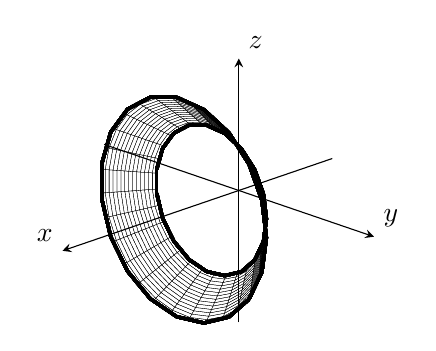
\begin{tikzpicture}
\begin{axis}[
  view={135}{20},
  axis lines=center,axis on top,
  ticks=none,set layers=default,axis equal,
  xlabel={$x$}, ylabel={$y$}, zlabel={$z$},
  xlabel style={anchor=south east},
  ylabel style={anchor=south west},
  zlabel style={anchor=south west},
  enlargelimits,
  tick align=inside,
  domain=0:2.00,
  samples=20,
  z buffer=sort,
]
  \def\a{0.8}
  \def\b{0.5}
  \def\c{0.5}
  \def\umax{1}

  \addplot3[
      mesh,
      samples=15,
      samples y=30,
      domain=1:2,
      domain y=0:360,
      draw=black,
      line width=0.1pt,
  ]
  (
      {x},
      {(x + 1)*cos(y)},
      {(x + 1)*sin(y)}
  );
  \addplot3[
      mesh,
      domain=0:360,
      samples=20,
      very thick,
      black
  ]
  (
    { 1 },
    { 2*cos(x) },
    { 2*sin(x) }
  );
  \addplot3[
      mesh,
      domain=0:360,
      samples=20,
      very thick,
      black
  ]
  (
    { 2 },
    { 3*cos(x) },
    { 3*sin(x) }
  );
\end{axis}
\end{tikzpicture}
\end{center}
\subsubsection{Finding the Flux}
Because of the cylindrical symmetry around the $x$-axis, we would like to use cylindrical polars.
To do this, we can either relabel the axis as $(z, x, y)$ (noting that these should remain right handed), or we can just modify our definition of cylindrical polars to:
\[
  x = x,\ y = \rho \cos \phi,\ z = \rho \sin \phi
\]
We choose to parameterise the cone using $x,\ \phi$ with $\rho = \beta(x + 1)$ so:
\[
  \vec{x}(x, \phi) = (x, \beta(x + 1)\cos \phi, \beta(x + 1)\sin \phi)
\]
Note that although we are using cylindrical polars here, since this is a surface, it is parameterised by $x$ and $\phi$ only, $\rho$ is not an independent variable.

Using \cref{dSFormula}, the vector surface element is:
\[
  \d{\vec{S}} = \pm \begin{pmatrix}
  1 \\
  \beta \cos \phi \\
  \beta \sin \phi \\
  \end{pmatrix} \times \begin{pmatrix}
  0 \\
  -\beta(x + 1)\sin \phi \\
  \beta(x + 1) \cos \phi \\
  \end{pmatrix} \d{x}\d{\phi} = \pm \begin{pmatrix}
  \beta^2(x + 1) \\
  -\beta(x + 1)\cos \phi \\
  -\beta(x + 1)\sin \phi \\
  \end{pmatrix} \d{x}\d{\phi}
\]
We need the $-$ sign to ensure that $\d{\vec{S}}$ points away from the $x$-axis.

Therefore, the flux $\mathscr{F}_S$ is:
\begin{align*}
  \mathscr{F}_S &= \int_{x = 1}^{2} \int_{\phi = 0}^{2\pi} \begin{pmatrix}
  x \\
  \beta(x + 1)\cos \phi \\
  \beta(x + 1)\sin \phi \\
  \end{pmatrix} \cdot \begin{pmatrix}
  -\beta^2 (x + 1) \\
  \beta(x + 1)\cos \phi \\
  \beta(x + 1)\sin \phi \\
  \end{pmatrix} \d{x} \d{\phi} \\
                &= \int_{x = 1}^{2} \int_{\phi = 0}^{2\pi} \beta^2(x + 1) \d{x} \d{\phi} = 5 \pi \beta^2
\end{align*}
\subsubsection{Verifying Result}
To verify this result using the divergence theorem, we need to turn $S$ into a \textit{closed surface} since it currently is not.
We can do this by adding two planar caps at $x = 1$ and $x = 2$.
Let $V$ be the enclosed volume by the caps and the original surface.
Luckily, the direction of the normals/$\d{\vec{S}}$ we used earlier are outwards from $V$ which is consistent with what we require for the divergence theorem.

Let the fluxes through the caps be $\mathscr{F}_1$ and $\mathscr{F}_2$ for the cap at $x = 1$ and $x = 2$ respectively.
Using the divergence theorem, since $\nabla \vec{F} = 3$, we have:
\[
  \int_{V} \nabla \cdot \vec{F} \d{V} = \mathscr{F}_{S} + \mathscr{F}_1 + \mathscr{F}_2 \implies \mathscr{F}_S = \int_{V} 3 \d{V} - \mathscr{F}_1 - \mathscr{F}_2
\]
For the first integral, we can either find three times the volume of the frustum or evaluate it directly, noting that $|J| = \rho$:
\begin{align*}
  \int_{V} 3 \d{V} &= \int_{x = 1}^{2} \int_{\rho = 0}^{\beta(x + 1)} \int_{\phi = 0}^{2\pi} 3\rho \d{\phi} \d{\rho} \d{x} \\
                   &= 6\pi \int_{1}^{2} \frac{1}{2}\beta^2(x + 1)^2 \d{x} = 19\pi \beta^2
\end{align*}
To find $\mathscr{F}_1$, the normal of the end cap at $x = 1$ is $\vec{n} = (-1, 0, 0)$ and so:
\[
  \mathscr{F}_1 = \int\limits_{\substack{x = 1 \\ y^2 + z^2 \leq 4\beta^2}} \begin{pmatrix}
  x \\
  y \\
  z \\
  \end{pmatrix} \cdot \begin{pmatrix}
  -1 \\
  0 \\
  0 \\
  \end{pmatrix} \d{y} \d{z} = -\int\limits_{y^2 + z^2 \leq 4\beta^2}  \d{y} \d{z} = -\pi(2\beta)^2
\]
since the area of the cap is $\pi(2\beta)^2$.

Similarly for the other cap, however here $\vec{n} = (1, 0, 0)$:
\[
  \mathscr{F}_2 = \int\limits_{\substack{x = 2 \\ y^2 + z^2 \leq 9\beta^2}} \begin{pmatrix}
  x \\
  y \\
  z \\
  \end{pmatrix} \cdot \begin{pmatrix}
  1 \\
  0 \\
  0 \\
  \end{pmatrix} \d{y} \d{z} = \int\limits_{y^2 + z^2 \leq 9\beta^2} 2 \d{y} \d{z} = 2\pi(3\beta)^2
\]
Finally:
\[
  \mathscr{F}_S = \pi \beta^2(19 - 4 - 19) = 5\pi \beta^2
\]
which is the same result as calculating the flux directly.
\subsection{Multiple Boundary Surfaces}
If $V$ contains one or more holes, then $\partial V$ will consist of two or more boundary surfaces.
To apply the divergence theorem, we need the normals to point outwards of $V$, so the normals will point into the holes.
For example, in this cross-section of a volume $V$ with boundary surfaces $S_1$ and $S_2$:
\begin{center}
\begin{tikzpicture}[>=stealth]
  \draw[thick, fill=gray!50] (-1,1) to[closed, curve through = { (-0.5, 1.3) (0, 1.8) (1, 1.9) (2.5, 0) (1.2, -1.9) (0, -1.6) }] (-1, -1);

  \draw[thick, fill=white, scale=0.3] (-1,1) to[closed, curve through = { (-0.5, 1.3) (0, 1.8) (1, 1.9) (2.5, 0) (1.2, -1.9) (0, -1.6) }] (-1, -1);

  \node at (2, 1.8) {$S_1$};
  \node at (0.7, 0.7) {$S_2$};
  \node at (1.5, -0.6) {$V$};
  \draw[thick, ->] (-0.45, 0) -- (-0, 0) node[below] {$\vec{n}$};
  \draw[thick, ->] (2.15, 1) -- (2.8, 1.45) node[right] {$\vec{n}$};
\end{tikzpicture}
\end{center}
We saw in \cref{greensMultipleBoundaries} that having multiple boundaries can allow us to traverse around a discontinuity in the domain.
A similar technique can also be applied using the divergence theorem by removing a small volume around the singularity to avoid integrating over it.
\begin{example}[Spherical Annulus]
  Apply the divergence theorem to a spherical annulus $V = \{\vec{x} \in \R^3: a < |\vec{x}| < b\}$.

  $\partial V$ consists of two spheres, $|\vec{x}| = a$ and $|\vec{x}| = b$.
  For the normals to point outwards of $V$, we need $\d{\vec{S}} = \vec{e}_r \d{S}$ on $|\vec{x}| = b$ but $\d{\vec{S}} = -\vec{e}_r \d{S}$ on $|\vec{x}| = a$.

  Hence:
  \[
    \int_{V} \nabla \cdot \vec{F} \d{V} = \int_{|\vec{\vec{x}}| = b} \vec{F}(\vec{x}) \cdot \vec{e}_r \d{S} - \int_{|\vec{x}| = a} \vec{F}(\vec{x}) \cdot \vec{e}_r \d{S}
  \]
\end{example}
\begin{remark}[Warning]
  Suppose we have a volume $V$ with outer surface $S_1$ and inner surface $S_2$.

  Some people would write the divergence theorem as:
  \[
    \int_{V} \nabla \cdot \vec{F} \d{V} = \int_{S_1} \vec{F}\cdot \d{\vec{S}} + \int_{S_2} \vec{F} \cdot \d{\vec{S}}
  \]
  with $\d{\vec{S}}$ pointing out of $V$ in both cases, that is outwards for $S_1$ and inwards for $S_2$.

  Whereas others would write:
  \[
    \int_{V} \nabla \cdot \vec{F} \d{V} = \int_{S_1} \vec{F} \cdot \d{\vec{S}} - \int_{S_2} \vec{F} \cdot \d{\vec{S}}
  \]
  with $\d{\vec{S}}$ being outwards from both $S_1$ and $S_2$.

  It is important to make sure you specify what convention your are using.
\end{remark}
\subsection{Connection to Other Integral theorems}
\nonexaminable
We can show that Green's Theorem in the plane \cref{greensTheorem} is a special case in 2D of the Divergence theorem.
If we let $\vec{F} = (Q, -P, 0)$, then the left hand side of Green's Theorem in the plane is:
\[
  \int_{A} \left(\pderiv{Q}{x} - \pderiv{P}{y}\right) \d{A} = \int_{A} \nabla \cdot \vec{F} \d{A}
\]
The right hand side is:
\[
  \oint_{C} (P \d{x} + Q \d{y}) = \oint_{C} \vec{F} \cdot \begin{pmatrix}
  \d{y} \\
  -\d{x} \\
  0 \\
  \end{pmatrix} = \oint \vec{F} \cdot \vec{n} \d{s}
\]
where $\vec{n} \d{s} = (\d{y, -\d{x}, 0})$ and $\d{s}$ is the infinitesimal arc length (i.e. the equivalent of $\d{S}$ in 1D).
Since $\vec{n}$ is perpendicular to $\d{\vec{x}} = (\d{x}, \d{y}, 0)$, and points in the correct direction, it is an outwards normal.
So by the divergence theorem, both sides are equal.

So the Divergence Theorem implies Greens Theorem in the plane, which in turn implies Stokes' Theorem.
In fact, they are all the same theorem in the differential geometry of manifolds, confusingly, also called Stokes' Theorem that states:
\[
  \int_{\Omega}  \d{\eta} = \int_{\partial \Omega} \eta
\]
where $\eta$ is a differential form, $\d{\eta}$ its exterior derivative and $\Omega$ an orientable manifold.
\section{Scalar Potentials for Irrotational Vector Fields}
\label{scalarPotentials}
In \cref{conservativeFields}, we stated that in a simply connected domain, an irrotational vector field is conservative.
That is, if $\nabla \cdot \vec{F} = \vec{0}$ everywhere in a simply connected domain $\mathscr{D}$, then there exists a single valued scalar potential $f$ such that $\vec{F} = \nabla f$.
We now have the tools to prove this assertion.
\begin{proof}
  We first need to show that if $\oint \vec{F} \cdot \d{\vec{x}} = 0$ for all closed curves $C$ then $\int_{\vec{a}}^{\vec{b}} \vec{F} \cdot  \d{\vec{x}}$ is path independent.
  Consider two any two possible paths $C_1$, $C_2$ from $\vec{a}$ to $\vec{b}$ and let $C = C_1 - C_2$.
  Since $C$ is a closed curve, we have:
  \[
    \oint \vec{F} \cdot \d{\vec{x}} = 0 \implies \int_{C_1} \vec{F} \cdot \d{\vec{x}} - \int_{C_2} \vec{F} \cdot  \d{\vec{x}} = 0
  \]
  and so the integrals over any two possible paths must be the same, as required.

  We can now prove the main result.
  Given an irrotational vector field $\vec{F}$, and an arbitrary closed curve $C$, let $S$ be a surface that spans $C$, that is, $C = \partial S$.
  By Stokes' Theorem $\int_{S} \nabla \times \vec{F} \cdot \d{\vec{S}} = \oint \vec{F} \cdot \d{\vec{x}} = 0$, and so by the above, the line integral of $\vec{F}$ is path independent.

  Since the line integral is path independent, we can define the single valued the scalar function:
  \[
    f(\vec{x}) = \int_{\vec{x}_0}^{\vec{x}} \vec{F} \cdot \d{\vec{x}}
  \]
  Where $\vec{x}_0$ is an arbitrary fixed point within the domain.
  Changing $\vec{x}_0$ would just shift $f$ by a constant which would just disappear upon taking grad.

  Consider:
  \[
    f(\vec{x} + \delta \vec{x}) - f(\vec{x}) = \int_{\vec{x}}^{\vec{x} + \delta \vec{x}}  \vec{F} \cdot \d{\vec{x}} = \vec{F}(\vec{x}) \cdot \delta \vec{x} + O(|\delta \vec{x}|^2)
  \]
  So in the limit as $\delta \vec{x} \to \vec{0}$, $\d{f} = f(\vec{x} + \d{\vec{x}}) - f(\vec{x}) = \vec{F} \cdot \d{\vec{x}}$.
  In \cref{infinitesimalsGrad}, we saw that we can define $\nabla f$ to be the unique vector such that $\d{f} = (\nabla f) \cdot \d{\vec{x}}$ for all $\d{x}$, therefore, we have $\vec{F} = \nabla f$, as required.
\end{proof}
\begin{remark}[Use of Simply Connectedness]
  \nonexaminable
  Here, we used simply connectedness to guarantee the existence of a surface $S$ that span $C$.
  If the domain $\mathscr{D}$ is not simply connected, then there are some closed curves that cannot be spanned by a surface lying entirely in $\mathscr{D}$.
\end{remark}
\section{Coordinate Independent Definitions of Vector Differential Operators}
\nonexaminable
Earlier, we defined grad with respect to the standard basis, but also in a coordinate independent way, using $\d{f} = \nabla f \cdot \d{\vec{x}}$.
However, we still only have definitions for div and curl using the standard basis.

\subsubsection{Divergence}
It can be shown using the Divergence Theorem (\cref{divergenceTheorem}) that:
\[
  \at{\nabla \cdot \vec{F}}{\vec{x}} = \lim_{\varepsilon \to 0} \frac{1}{V_\varepsilon} \int_{\partial V_\varepsilon} \vec{F}\cdot \d{\vec{S}}
\]
where $V_\varepsilon$ is a small volume (or the volume of such a volume) of maximum linear dimension $\varepsilon$ that contains $\vec{x}$.
\subsubsection{Curl}
It can be shown using Stokes' Theorem (\cref{stokesTheorem}) that:
\[
  \at{\vec{k} \cdot (\nabla \times \vec{F})}{\vec{x}} = \lim_{\varepsilon \to 0} \frac{1}{S_\varepsilon(\vec{k})} \oint_{\partial S_\varepsilon(\vec{k})} \vec{F} \cdot \d{\vec{x}}
\]
where $S_\varepsilon(\vec{k})$ is a small open surface (or the area of such a surface) of maximum linear dimension $\varepsilon$ that contains $\vec{x}$ and has normal $\vec{n} = \vec{k}$ at $\vec{x}$.
We can then find the components with respect to an arbitrary orthonormal basis by taking $\vec{k}$ to be each of the basis vectors in turn.
\subsubsection{Finding Div and Curl in Orthogonal Curvilinear Coordinate Systems}
In \cref{generalCurvilinearOperators}, we saw divergence and curl for an arbitrary orthogonal curvilinear coordinate system.
The above two coordinate independent forms can be used to derive these identities, the details of which are not included in this course.
\section{Green's Identities and Other Corollaries}
\subsection{Green's Identities}
\begin{theorem}[Green's First Identity]
  If $\phi$ and $\psi$ are scalar fields defined in a closed volume $V$ with surface $\partial V$ and outward normal $\vec{n}$, then:
  \label{greensFirst}
  \[
    \int_{V} (\phi \nabla^2 \psi + \nabla \phi \cdot \nabla \psi) \d{V} = \int_{\partial V} \phi \nabla \psi \cdot \d{\vec{S}}
  \]
\end{theorem}
\begin{proof}
  Let $\vec{F} = \phi \nabla \psi$ using an identity from \cref{vectorIdentities}, we have:
  \begin{align*}
    \nabla \cdot \vec{F} = \nabla \cdot (\phi \nabla \psi) &= \phi (\nabla \cdot (\nabla \psi)) + \nabla \psi \cdot \nabla \phi \\
                                                           &= \phi \nabla^2 \psi + \nabla \phi \cdot \nabla \psi
  \end{align*}
  So the result follows using the divergence theorem (\cref{divergenceTheorem}).
\end{proof}
\begin{theorem}[Green's Second Identity]
  If $\phi$ and $\psi$ are scalar fields defined in a closed volume $V$ with surface $\partial V$ and outward normal $\vec{n}$, then:
  \label{greensSecond}
  \[
    \int_{V} (\phi \nabla^2 \psi - \psi \nabla^2 \phi) \d{V} = \int_{\partial V} (\phi \nabla \psi - \psi \nabla \phi) \cdot \d{\vec{S}}
  \]
\end{theorem}
\begin{proof}
  Proved in a similar fashion to Greens first identity, see Example Sheet 3.
\end{proof}
\begin{remark}[Notation]
  In these identities, since $\d{\vec{S}} = \vec{n} \d{S}$ (see \cref{vectorSurfaceElement}), multiple terms of the form $\nabla f \cdot \vec{n}$ appear, so we introduce the following notation for convenience:
  \[
    \pderiv{f}{\vec{n}} \equiv \nabla f \cdot \vec{n}
  \]
  This is the same as the directional derivative $D_{\vec{n}}f$ from \cref{directionalDerivative}.
  It is also sometimes written as $\pderiv{f}{n}$, that is, without notating $\vec{n}$ as a vector.
\end{remark}
Using this notation, Green's first identity (\cref{greensFirst}) becomes:
\[
  \int_{V} (\phi \nabla^2 \psi + \nabla \phi \cdot \nabla \psi) \d{V} = \int_{\partial V} \phi \pderiv{\psi}{\vec{n}} \d{S}
\]
Similarly, Green's second identity (\cref{greensSecond}) becomes:
\[
  \int_{V} (\phi \nabla^2 \psi - \psi \nabla^2 \phi) \d{V} = \int_{\partial V} \left(\phi \pderiv{\psi}{\vec{n}} - \psi \pderiv{\phi}{\vec{n}}\right) \d{S}
\]
\subsection{A Corollary of the Divergence Theorem}
We first need a lemma about dot products:
\begin{lemma}
  If $\vec{a} \cdot \vec{b} = \vec{a} \cdot \vec{c}$ for all $\vec{a} \in \R^3$, then $\vec{b} = \vec{c}$.
  \label{dotProdLemma}
\end{lemma}
\begin{proof}
  First, for any vectors $\vec{a}, \vec{b}, \vec{c}$ we have:
  \[
    \vec{a} \cdot \vec{b} = \vec{a} \cdot \vec{c} \implies \vec{a} \cdot (\vec{b} - \vec{c}) = 0 \implies \vec{a} \perp (\vec{b} - \vec{c})
  \]
  Suppose now that $\vec{a} \cdot \vec{b} = \vec{a} \cdot \vec{c}$ for all $\vec{a}$.
  This means that $(\vec{b} - \vec{c}) \perp \vec{a}$ for all $\vec{a}$, but the only vector orthogonal to every vector is $\vec{0}$ and so $\vec{b} = \vec{c}$.
\end{proof}
\begin{proposition}
  If $f$ is a scalar field then:
  \[
    \int_{V} \nabla f \d{V} = \int_{\partial V} f \d{\vec{S}}
  \]
\end{proposition}
\begin{remark}[Note]
  Although it may at first not look like it, both sides of this are vectors in $\R^3$, this is because $\nabla f \in \R^3$ and $\d{\vec{S}} \in \R^3$ as $\d{\vec{S}} = \vec{n}\d{S}$.
\end{remark}
\begin{proof}
  Consider the vector field $\vec{F} = f \vec{a}$ where $f$ is a scalar field and $\vec{a}$ is an arbitrary constant vector.
  Using an identity from \cref{vectorIdentities}, we have:
  \[
    \nabla \cdot \vec{F} = f \cancelto{0}{\nabla \cdot \vec{a}} + \vec{a} \cdot \nabla f = \vec{a} \cdot \nabla f
  \]
  and so, applying divergence theorem (\cref{divergenceTheorem}), we have:
  \begin{align*}
    \int_{V} \vec{a} \cdot \nabla f \d{V} &= \int_{\partial V} f \vec{a} \cdot \d{\vec{S}} \\
    \implies \vec{a} \cdot \int_{V} \nabla f \d{V} &= \vec{a} \cdot \int_{\partial V} f \d{\vec{S}} \text{ since $\vec{a}$ is constant}
  \end{align*}
  Since $\vec{a}$ was arbitrary, we can use \cref{dotProdLemma} to yield the result.
\end{proof}
\begin{example}
  Integrate $\nabla f$ where $f(\vec{x}) = xyz$ in the cube $V: 0 \leq x, y, z \leq 2$ and confirm the result using the above identity.

  Firstly, $\nabla f = (yz, xz, xy)$.
  We can then integrate component-wise:
  \[
    \int_{V} \nabla f \d{V} = \begin{pmatrix}
    \int_{V} yz \d{V} \\
    \int_{V} xz \d{V} \\
    \int_{V} xy \d{V} \\
    \end{pmatrix} = \begin{pmatrix}
    8 \\
    8 \\
    8 \\
    \end{pmatrix}
  \]
  Since $\int_{V} yz \d{V} = \int_{0}^{2} \int_{0}^{2} \int_{0}^{2} yz \d{x} \d{y} \d{z} = 8$ and similarly for the other components by symmetry.

  Continued next lecture.
\end{example}
\end{document}
